\section{Theorie}
\label{sec:Theorie}

\subsection{Zielsetzung}
\label{subsec:zielsetzung}
Ziel des im Folgenden beschriebenen Versuchs ist es,
mit Hilfe des Prinzips der Röntgenreflektrometrie
einen Nanometer-dicken Polystyrolfilm, der auf einen Silizium
Wafer aufgetragen ist, zu untersuchen.
Dazu wird ein D8-Labordiffraktometer zunächst justiert und anschließend zu
Messungen verwendet, aus deren Ergebnissen dann Schichtdicke, Rauigkeit und
Elektronendichte der Probe bestimmt werden.


\subsection{Brechung von Röntgenstrahlung an einer Grenzfläche}
\label{subsec:einschicht}
Um das Prinzip der Röntgenreflektrometrie zu verstehen ist es notwendig,
sich mit der Brechung von Röntgenstrahlung an einer Grenzfläche auseinander
zu setzen.
% Brechungsindex
Bei Röntgenstrahlung handelt es sich um elektromagnetische Wellen, deren
Wellenlängen in einem Bereich von circa $\SI{0.1}{\angstrom}$ bis
$\SI{10}{\angstrom}$ liegen.
Um den Übergang einer solchen Welle von einem Medium mit Brechungsindex $n_{1}$
in ein zweites mit Brechungsindex $n_{2}$ (siehe Abbildung \ref{fig:einschicht})
zu beschreiben, kann das Brechungsgesetz nach Snellius
\begin{align}
  n_{1} \cos\alpha_{\text{i}} = n_{2} \cos\alpha_{\text{t}}
  \label{eqn:snellius}
\end{align}
verwendet werden. Dabei bezeichnet $\alpha_{\text{i}}$ den Einfallswinkel
und $\alpha_{\text{t}}$ den Winkel unter dem die Strahlung gebrochen wird
(vgl. Abbildung \ref{fig:einschicht}). Es wird eine ideale glatte Grenzfläche
angenommen. \\

\FloatBarrier
\begin{figure}
  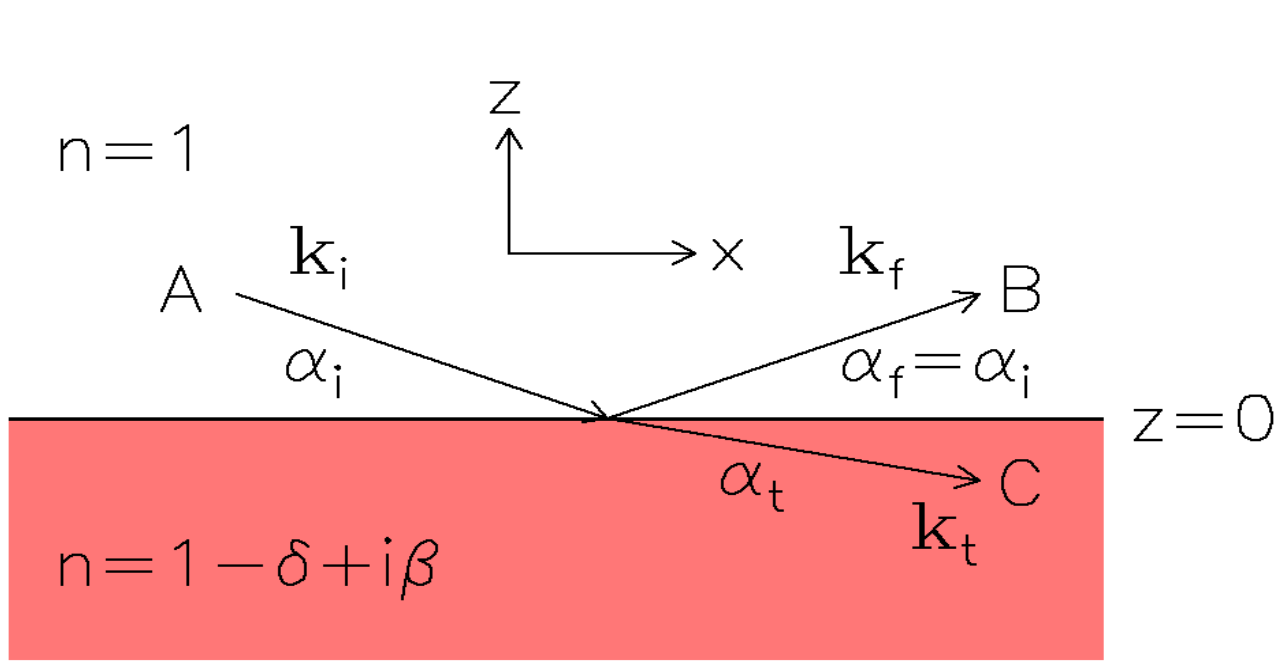
\includegraphics[width=\textwidth]{bilder/einschicht.png}
  \caption{Übergang einer elektromagnetischen Welle vom Vakuum in ein
            anderes Medium und dabei auftretetende Reflexion und Transmission.\cite{sample}}
  \label{fig:einschicht}
\end{figure}
\FloatBarrier

In Abbildung \ref{fig:einschicht} wird für das Ursprungsmedium das Vakuum gewählt,
sodass gilt $n_{1} = 1$. Für den Brechungsindex $n_{2}$ des anderen Mediums,
wird eine komplexe Zahl
\begin{align}
  n_{2} = \alpha + i \beta& &\text{mit } \alpha, \beta \in \mathbb{N}
  \label{eqn:komplexerindex}
\end{align}
gewählt. Der Realteil $\alpha$ beinhaltet die Informationen bezüglich der eigentlichen
Brechung und der Imaginarteil $\beta$ die Dämpfung der Welle im Medium. Für Röntgenstrahlung
gilt typischerweise $\alpha < 1$. Dies liegt daran, dass der reele
Brechungsindex das Verhältnis von Lichtgeschwindigkeit im Medium zu der im Vakuum
misst und für Röntgenstrahlung die Phasengeschwindigkeit im Medium
schneller sein kann als die Vakuumlichtgeschwindigkeit $c_{0}$.
Da der Realteil von $n$ den Wert $1$ nur um sehr kleine Werte
$\delta \sim 10^{-6}$ unterschreitet, wird die Formulierung
$\alpha = 1 - \delta$ gewählt,
sodass aus Gleichung \eqref{eqn:komplexerindex},
\begin{align}
  n_{2} = 1 - \delta + i \beta
  \label{eqn:komplexerindexdelta}
\end{align}
wird.

% kritischer Winkel
Anhand des Brechungsgesetzes \eqref{eqn:snellius} wird klar , dass ein Winkel
$\alpha_\text{{crit.}} = \arccos\left( n_{2} \right)$ existiert,
ab dem die Welle nicht in das zweite Medium eintritt,
also total refelektiert wird.
Damit überhaupt transmittierte Strahlung auftritt muss also gelten,
$\alpha_{\text{i}} > \alpha_{\text{crit.}}$.


% fresnel -> transmissions/reflektions amplituden -> Fresnelreflektivitaet



% dag
\subsection{Brechung von Röntgenstrahlung in Mehrschichtsystemen}
\label{subsec:mehrschicht}
Im Folgenden wird nun nicht mehr 
die Röngenreflektivität
eins einschichtigen 
Mediums betrachtet sondern eines Mehrschichtsystem wie 
beispielsweise ein $\SI{800}{\angstrom}$ dicker Polystyrolfilm (PS) 
auf Silizium (Si). Die berechntet Röngenreflektivität dieses 
Systems ist in der Abbilung \ref{fig:mehrschicht} dargestellt. 

\begin{figure}
\centering
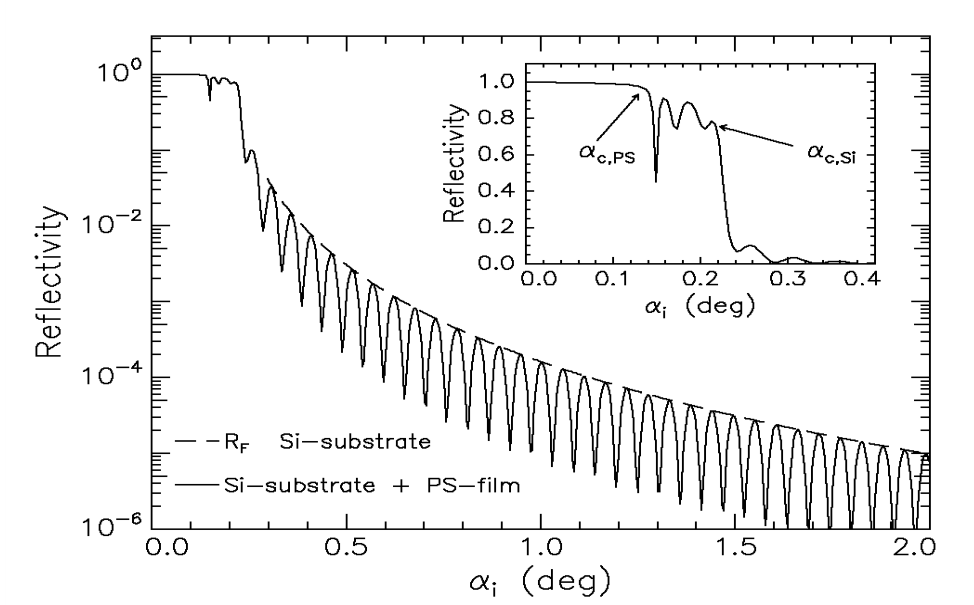
\includegraphics[widht = 0.7\textwidth]{bilder/mehrschicht_beispiel.PNG}
\caption{Berechnete Röngenreflektivität für $\lambda=\SI{1.54}{\angstrom} $ sowohl eines 
$\SI{800}{\angstrom}$ dicker Polystyrolfilm (PS) 
auf Silizium (Si)} als auch die reine Röngenreflektivität von Si ohne Film.
in Abhängigkeit des Einfallswinkel $\alpha_i$.\cite{sample}}
\label{fig:mehrschicht}
\end{figure}

Deutlich zu erkennen ist der Abfall in der Reflektivität wie schon 
bei einem Einschichtsystemen nach der Formel \ref{eqn??}.
  
Die Ozillation in der Reflektivität aus der Abbildung \ref{subsec:mehrschicht}
lassen sich auf konstruktive und destruktive Interferenzen in
der refelektiert Strahlung zurückführen.
Da bei einem Mehrschichtsystem mehr  
Grenzflächen, an denen Reflexion auftritt, exsistiern,
kömmt es zu einer Überlagerung der an unterschiedlichen Grenzflächen 
refelektierten Strahlen. 
Beträgt der Gangunterschied der Strahlen 
ein ungerades Vielfaches der halben Wellenlänge
kommt es zu einer destruktive Interferenzen und für gerade Vielfach 
liegt konstruktive Interferenzen vor.
Die so auftretetenden  
Modulationen in der Reflektionskurve 
werden auch "Kiessig-Ringe" gennant.
Für ein einfaches Modelle mit zwei 
Grenzschichten mit dem Schichtabstand $d$
ergibt sich der Zusammenhang
\begin{align}
  d = \frac{2\pi}{\Delta q_z} \approx \frac{\lambda}{2\Delta \alpha_i}.
\end{align}
Dabei ist $q$ der Wellenvetorübertrag für den gilt 
$\vec{q} = \vec{k}_f \vec{k}_i$ und welcher die z-Komponente $q_z=2k\sin \alpha_i$ besitzt  
Dabei sind $\Delta q_z$ und $\Delta\alpha_i$ Differenzen 
der jeweiligen
Werte zwischen zwei benachbarten Minima. % ????????

Für Mehrschichtsysteme mit Schichten
unterschiedlicher Brechungsindizes
ergibt sich auf Grund der Überlagerungen der reflektierten 
Strahlen eine  
komplizierte Reflektivität, für die der 
rekusiven Parratt-Algorithmus einen Lösungsansatz
liefert.
Der Parratt-Algorithmus geht von einem System 
wie in Abbildung \ref{fig:parratt_syst} dargestellt  
mit $N$ glatte Grenzflächen und somit $N+1$ Schichten 
aus. 

\begin{figure}
  \centering
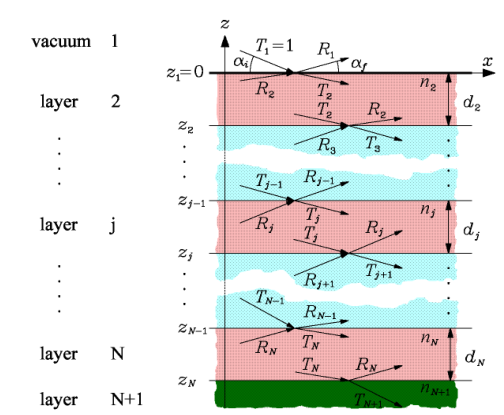
\includegraphics[\width=0.7\textwidth]{mehrschicht_parratt.PNG}
\caption{Beispiel System für den Parratt-Algorithmus 
mit $N+1$ Schichten und $N$ glatten Grenzflächen.\cite{sample}}
\label{fig:parratt_syst}
\end{figure}

Die erste Schicht ist das Vakuum mit Brechungsindex $n=1$ 
und die letzte Schicht ist das Substrat, welches als
unendlich dick angenommen wird.
Diese Annahme ist 
eine gute Nährung  
solange 
die Substratdicke größer gegenüber der  
Eindringtiefe ist.
Als Folge dessen existiert eine Startwert 
für den Parratt-Algorithmus, da
aus dem Substrat keine refektierte Strahlung $R_{N+1}$ 
existiert.
Für das Verhältnis von refelektierter und transmittierte Amplitude
$\mathrm{X}_j$ an der $j$-ten Grenzfläche liefert der 
Parratt-Algorithmus den Zusammenhang

\begin{align}
\mathrm{X}_j = \frac{\mathrm{R}_j}{\mathrm{T}_j} = \exp\left(-2\symup{i} \mathrm{k}_{z,j} \mathrm{z}_j\right) 
\frac{\mathrm{r}_{j,j+1} + \mathrm{X}_{j+1}\exp\left(2\symup{i} \mathrm{k}_{z,j+1} \mathrm{z}_j \right)}
{1 + \mathrm{r}_{j,j+1} + \mathrm{X}_{j+1}\exp\left(2\symup{i} \mathrm{k}_{z,j+1} \mathrm{z}_j \right)}.
\end{align}
Der koeffizienten $\mathrm{r}_{j,j+1}$ entspricht dabei 
der Fresnelreflektivität an der $j$-ten Grenzfläche
mit 
\begin{align}
  \mathrm{r}_{j,j+1} &= \frac{\mathrm{k}_{z,j}-\mathrm{k}_{z,j+1}}{\mathrm{k}_{z,j} + \mathrm{k}_{z,j+1}}
\intertext{und der z-komponente des Wellenvektors in der $j$-ten Schicht}
 \mathrm{k}_{z,j} &= \mathrm{k}\left(\mathrm{n}_j^2 - \cos^2\alpha_i\right)^{\sfrac{1}{2}}
\end{align}

% Reflektivitaet + Kiessig-Ringe


% rekursionszeug + Gesamtreflektivitaet


\subsection{Rauigkeit}
\label{subsec:rauigkeit}
Die zuvorher eingehende
Annahme, dass es sich bei alle betrachteten Grenzflächen um 
glatte Grenzflächen wird nun verworfen, da in 
der Realität bei Grenzflächen immer 
eine endliche Rauigkeit auftritt.
Wobei die Rauigkeit nur in z-Richtung bestimmen lässt, da 
bei Reflektivitätsmessungen mit einem 
Impulsübertrag senktecht zur Probenoberfläche das Signal 
keine Informationen laterale Oberflächenstruktur 
enthält.
Die Übergangsbereich zwischen zwei Schichten besitzen 
nun einen gemittelten Brechungsindex 
$\mathrm{n}(z)$, der für den Grenzfall 
glatter Grenzflächen, also geringer Rauigkeit, 
einer Heavisidefunktion \Theta(z) entspricht.
Mit einer 

Durch Rauigkeit Schmiert übergang aus 

Mit hilfe d



\cite{sample}
